% !TeX root = document.tex
% !TeX encoding = UTF-8 Unicode

\chapter{Controle do Sistema}%
\label{chapter:system-control}

Esse módulo permite que o usuário escreva testes utilizando a linguagem de
programação \textit{Python}. Dessa forma o usuário tem total liberdade para
controlar as saídas do sistema, e, por dispor de uma linguagem de programação
completa, possibilita o desenvolvimento de qualquer controlador. Embora ideal
para controle em malha fechada, também é útil para criar sinais complexos para a
malha aberta, além de permitir a aplicação de sinais diferentes em portas
diferentes.

A tela inicial do módulo, representada na Figura~\ref{fig:control1}, lista os
controladores salvos. As opções são as mesmas presentes no módulo Resposta do
Sistema (Capítulo~\ref{chapter:system-response}).

\begin{figure}[ht!]
    \centering
    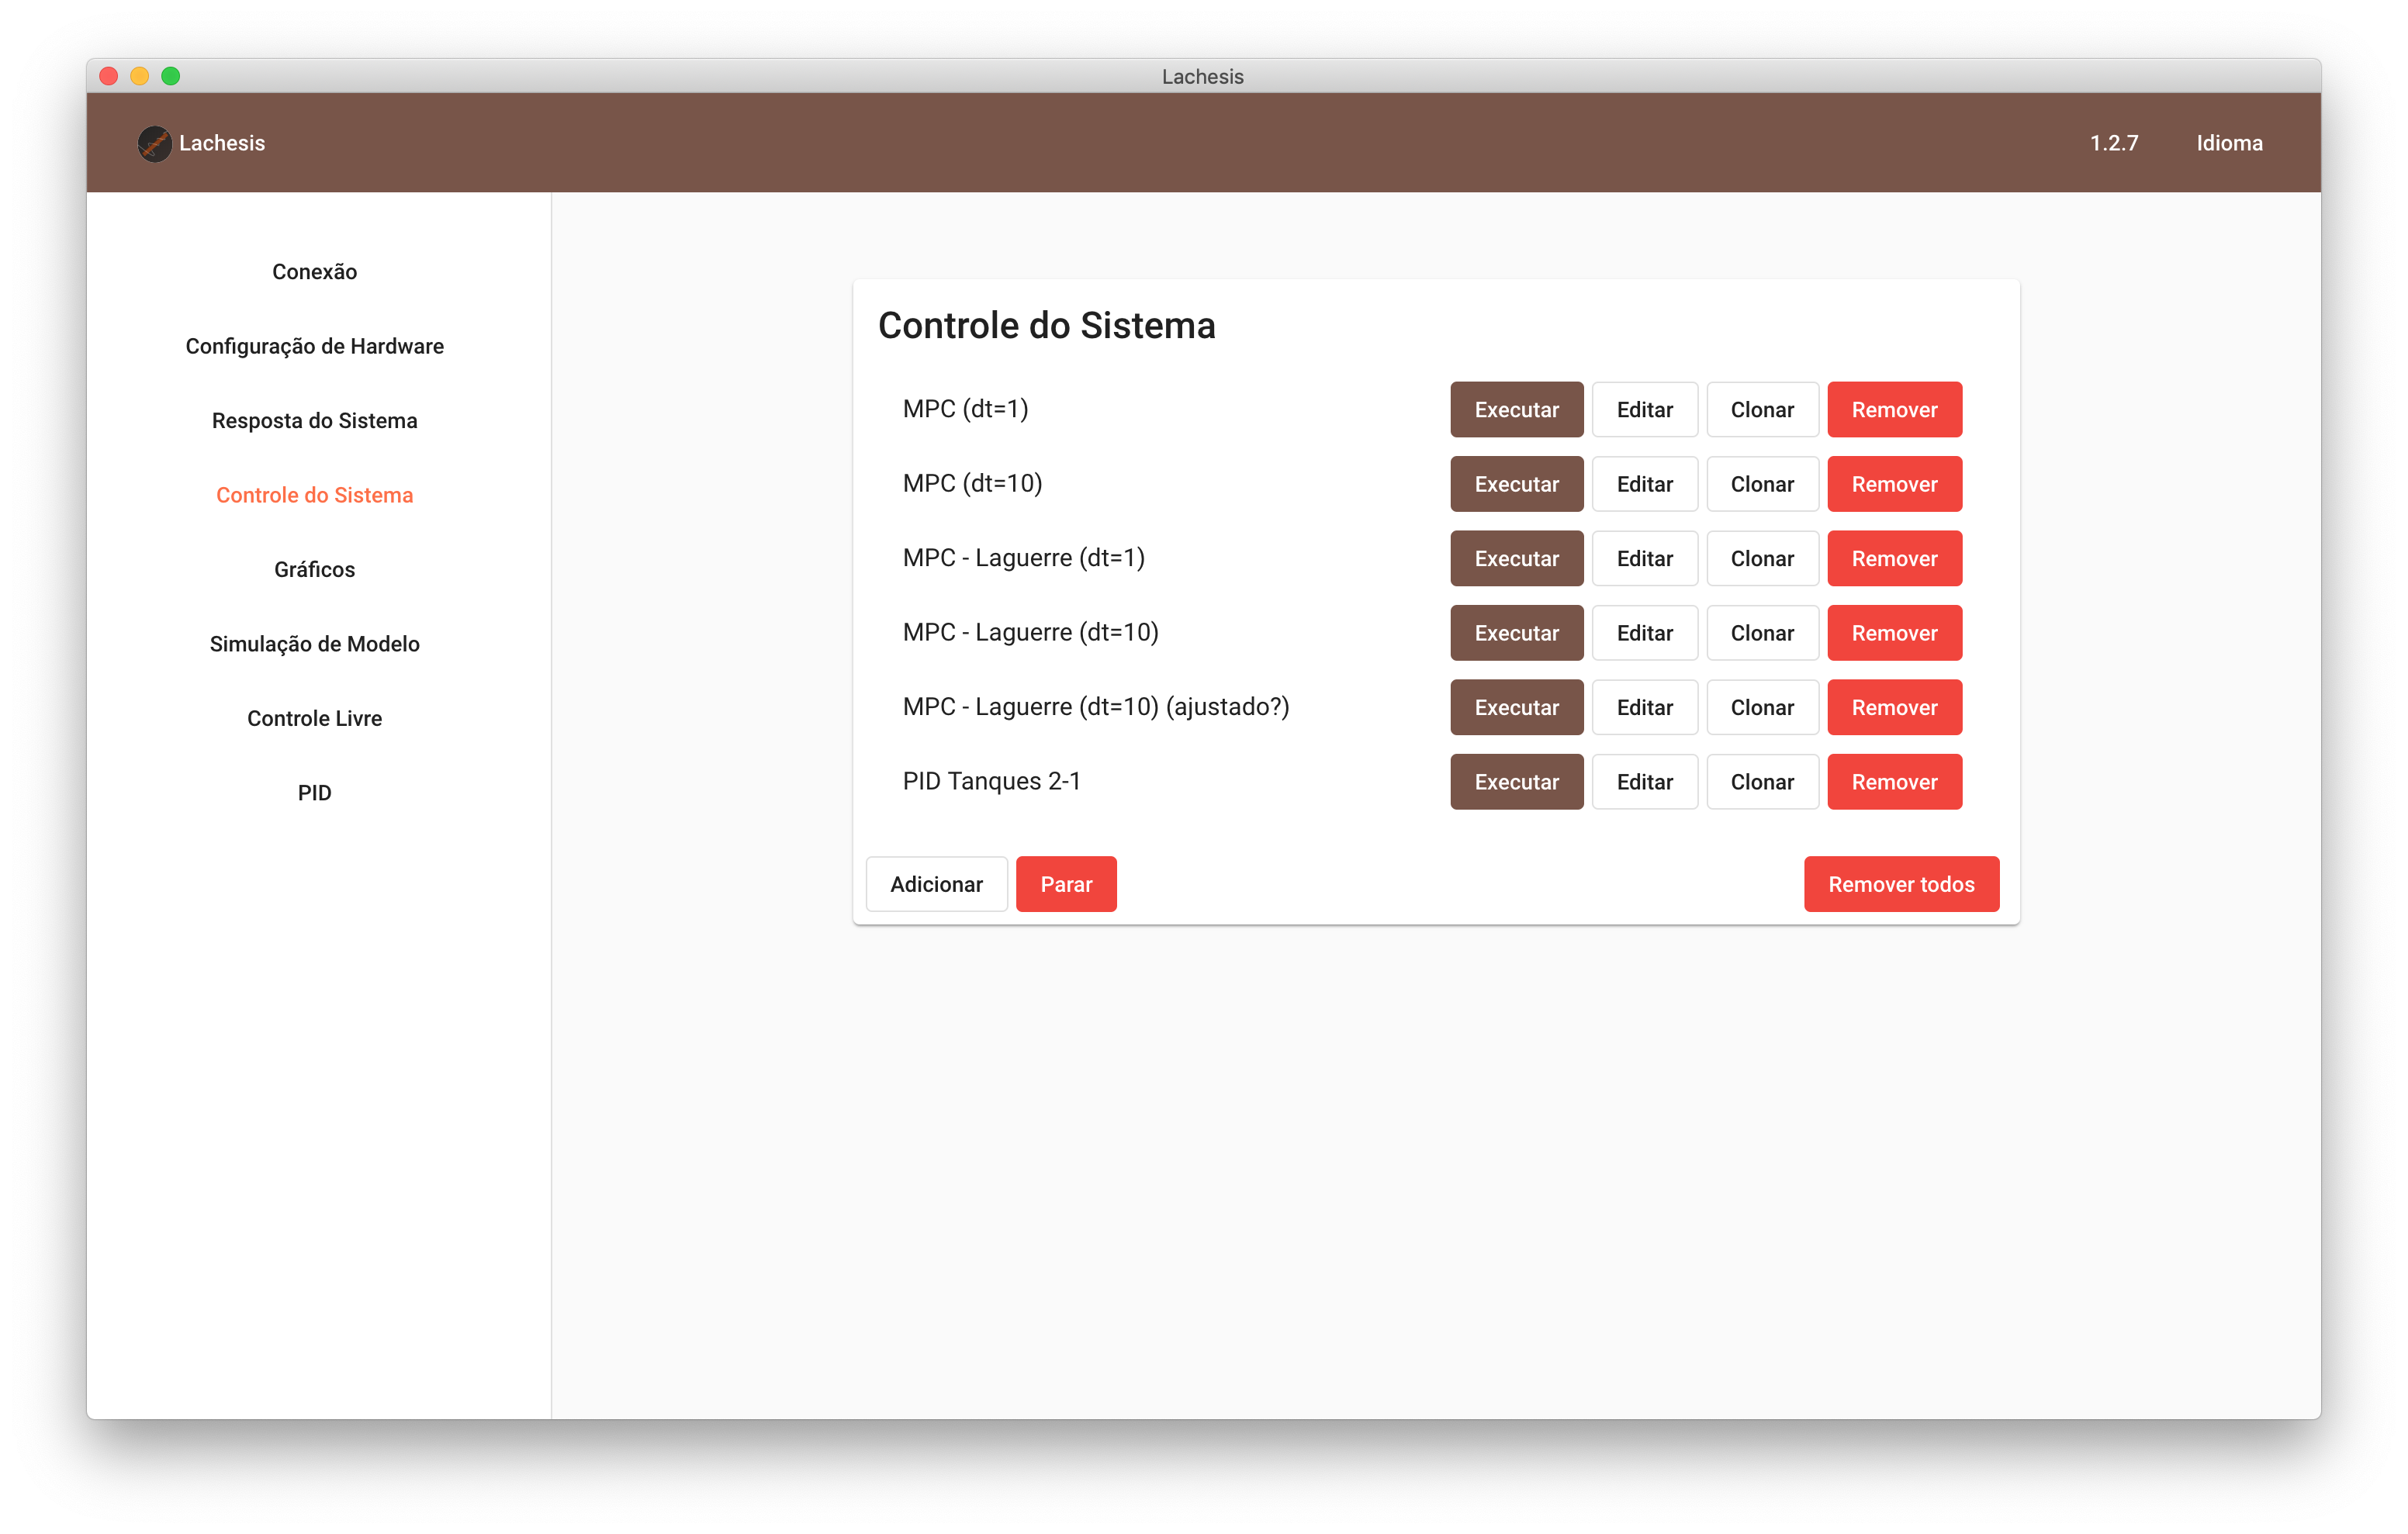
\includegraphics[width=0.9\textwidth]{imgs/control1}
    \caption[Módulo Controle do Sistema]{Módulo Controle do Sistema}%
    \label{fig:control1}
\end{figure}

Ao clicar em \textit{Adicionar} ou em \textit{Editar}, uma nova interface
(Figura~\ref{fig:control2}) se abre permitindo a edição do teste. No topo temos
os campos \textit{Nome}, assim como em \textit{Resposta do Sistema} e sendo
pertinente as mesmas recomendações, \textit{Tempo de amostragem} e \textit{Tempo
total de execução}, que é o tempo máximo que o teste será executado. O mesmo
pode ser interrompido precocemente por motivos de erro ou intertravamento.

\begin{figure}[ht!]
    \centering
    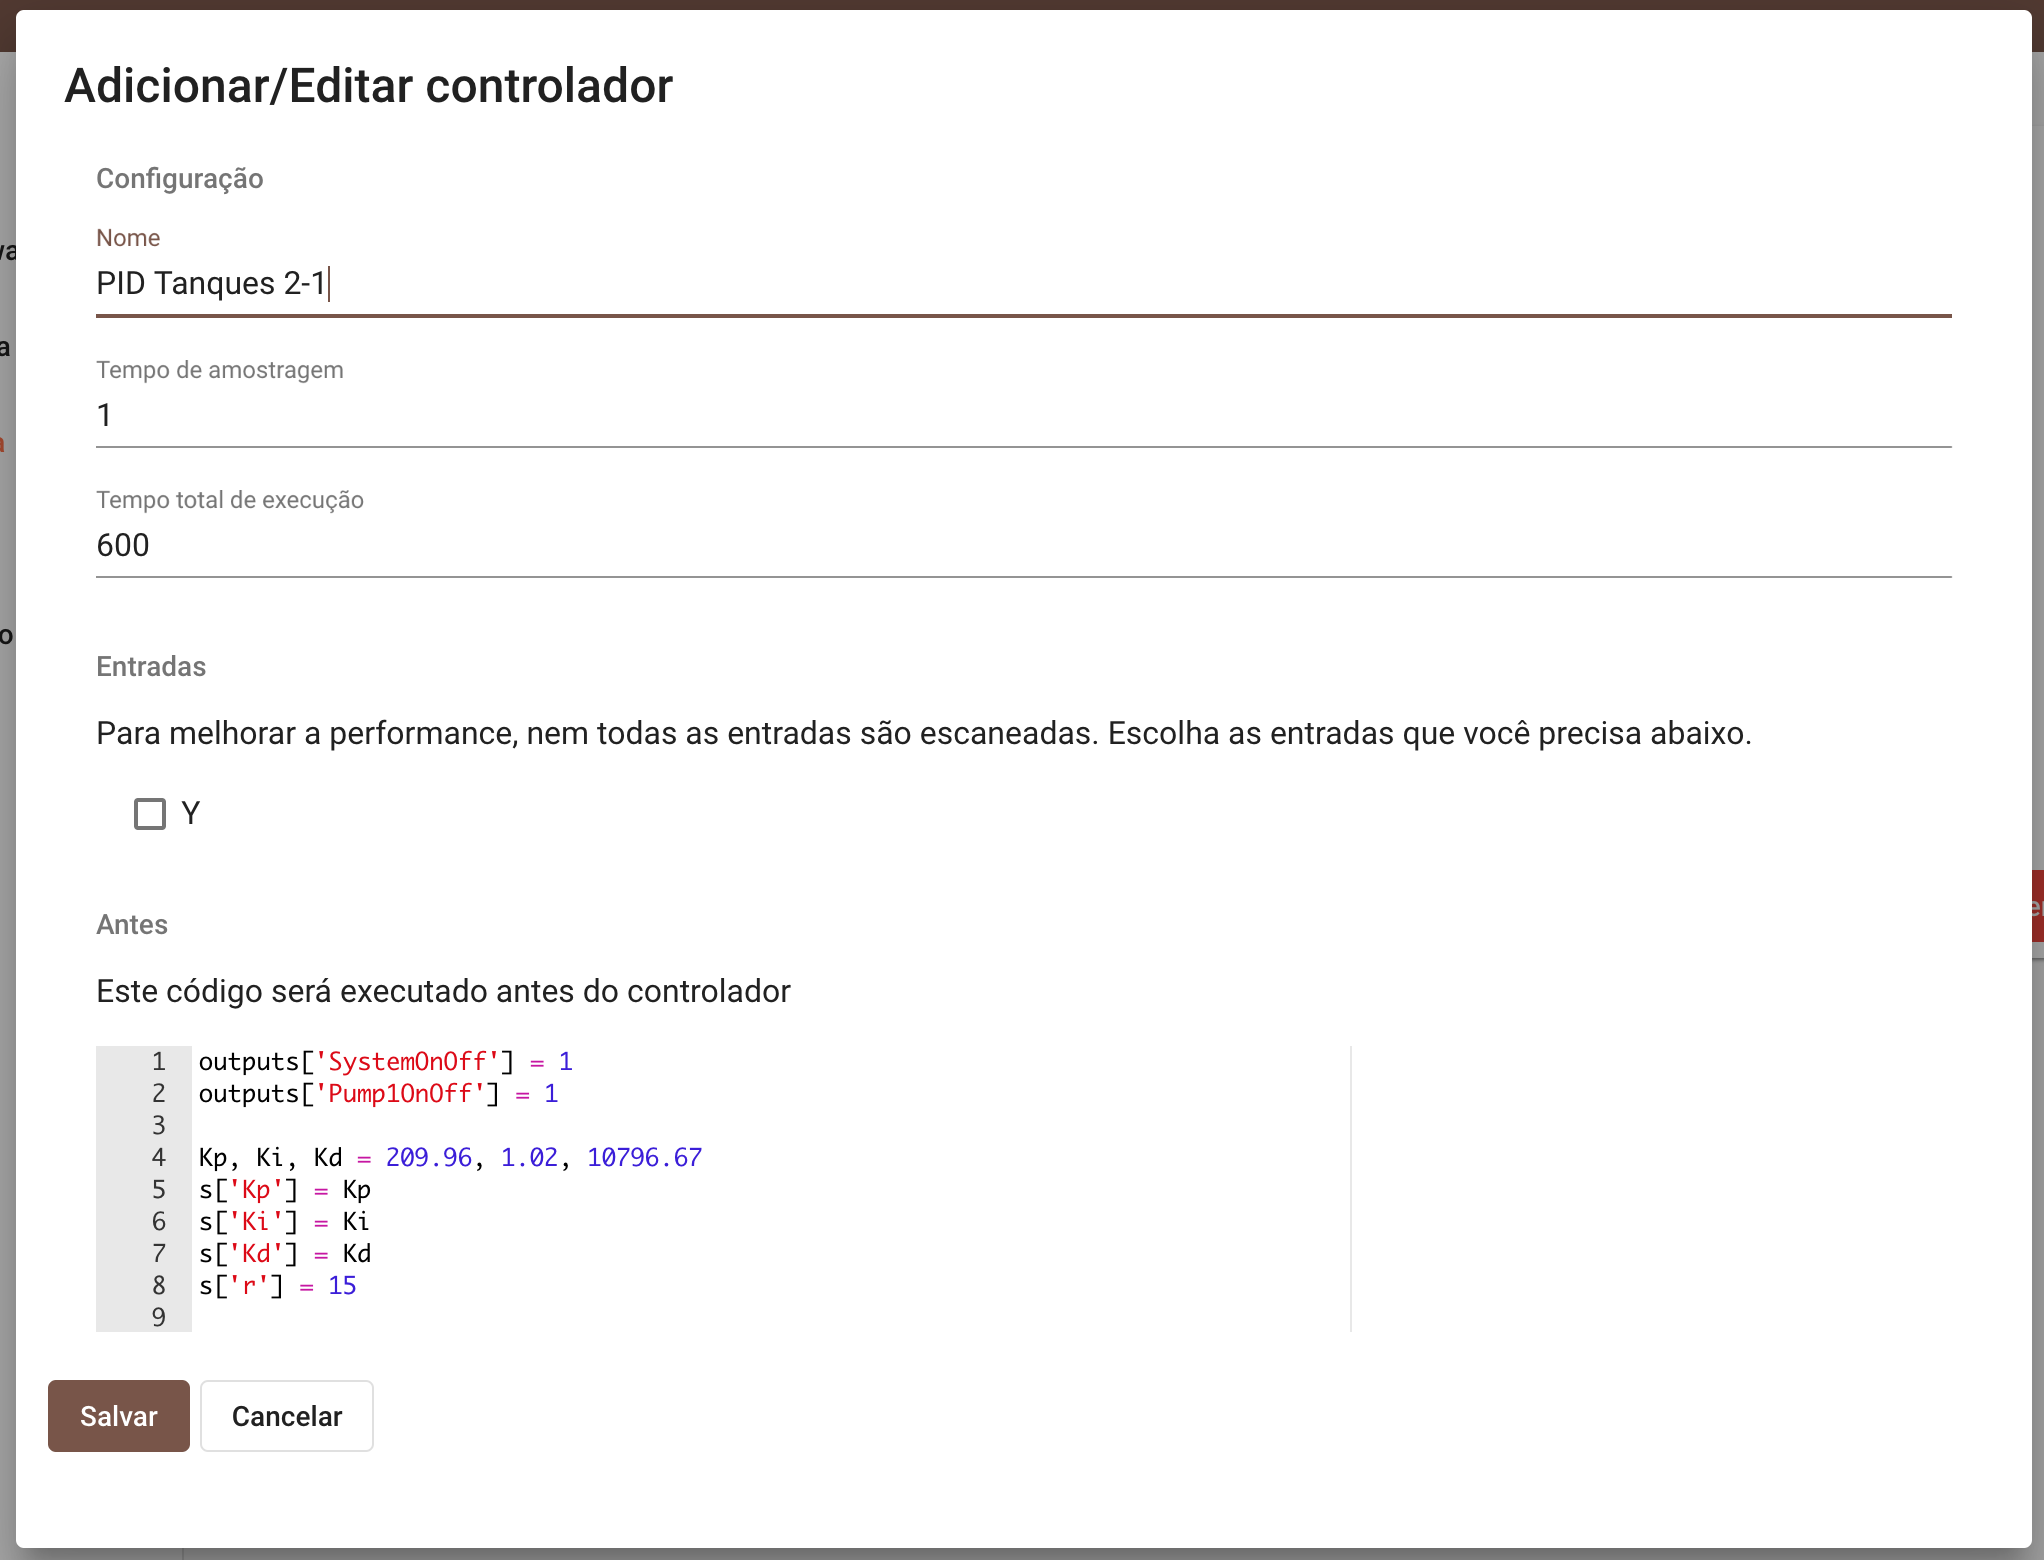
\includegraphics[width=0.9\textwidth]{imgs/control2}
    \caption[Edição de controlador]{Edição de controlador}%
    \label{fig:control2}
\end{figure}

Na seção \textit{Entradas} o usuário deve escolher as portas de entrada que
serão lidas. Apenas as portas selecionadas serão lidas e estarão disponíveis no
código. Isso evita ler informações desnecessárias e agiliza a execução do
código.

No campo \textit{Antes}, visto na Figura~\ref{fig:control3}, podemos inserir o
código que será executado uma vez antes do controlador iniciar. Esse campo é
ideal para calcular ganhos estáticos (como observadores ou \textit{MPC}) e para
salvar informações constantes e valores iniciais, como \(K_p\) ou \(x_0\).

\begin{figure}[ht!]
    \centering
    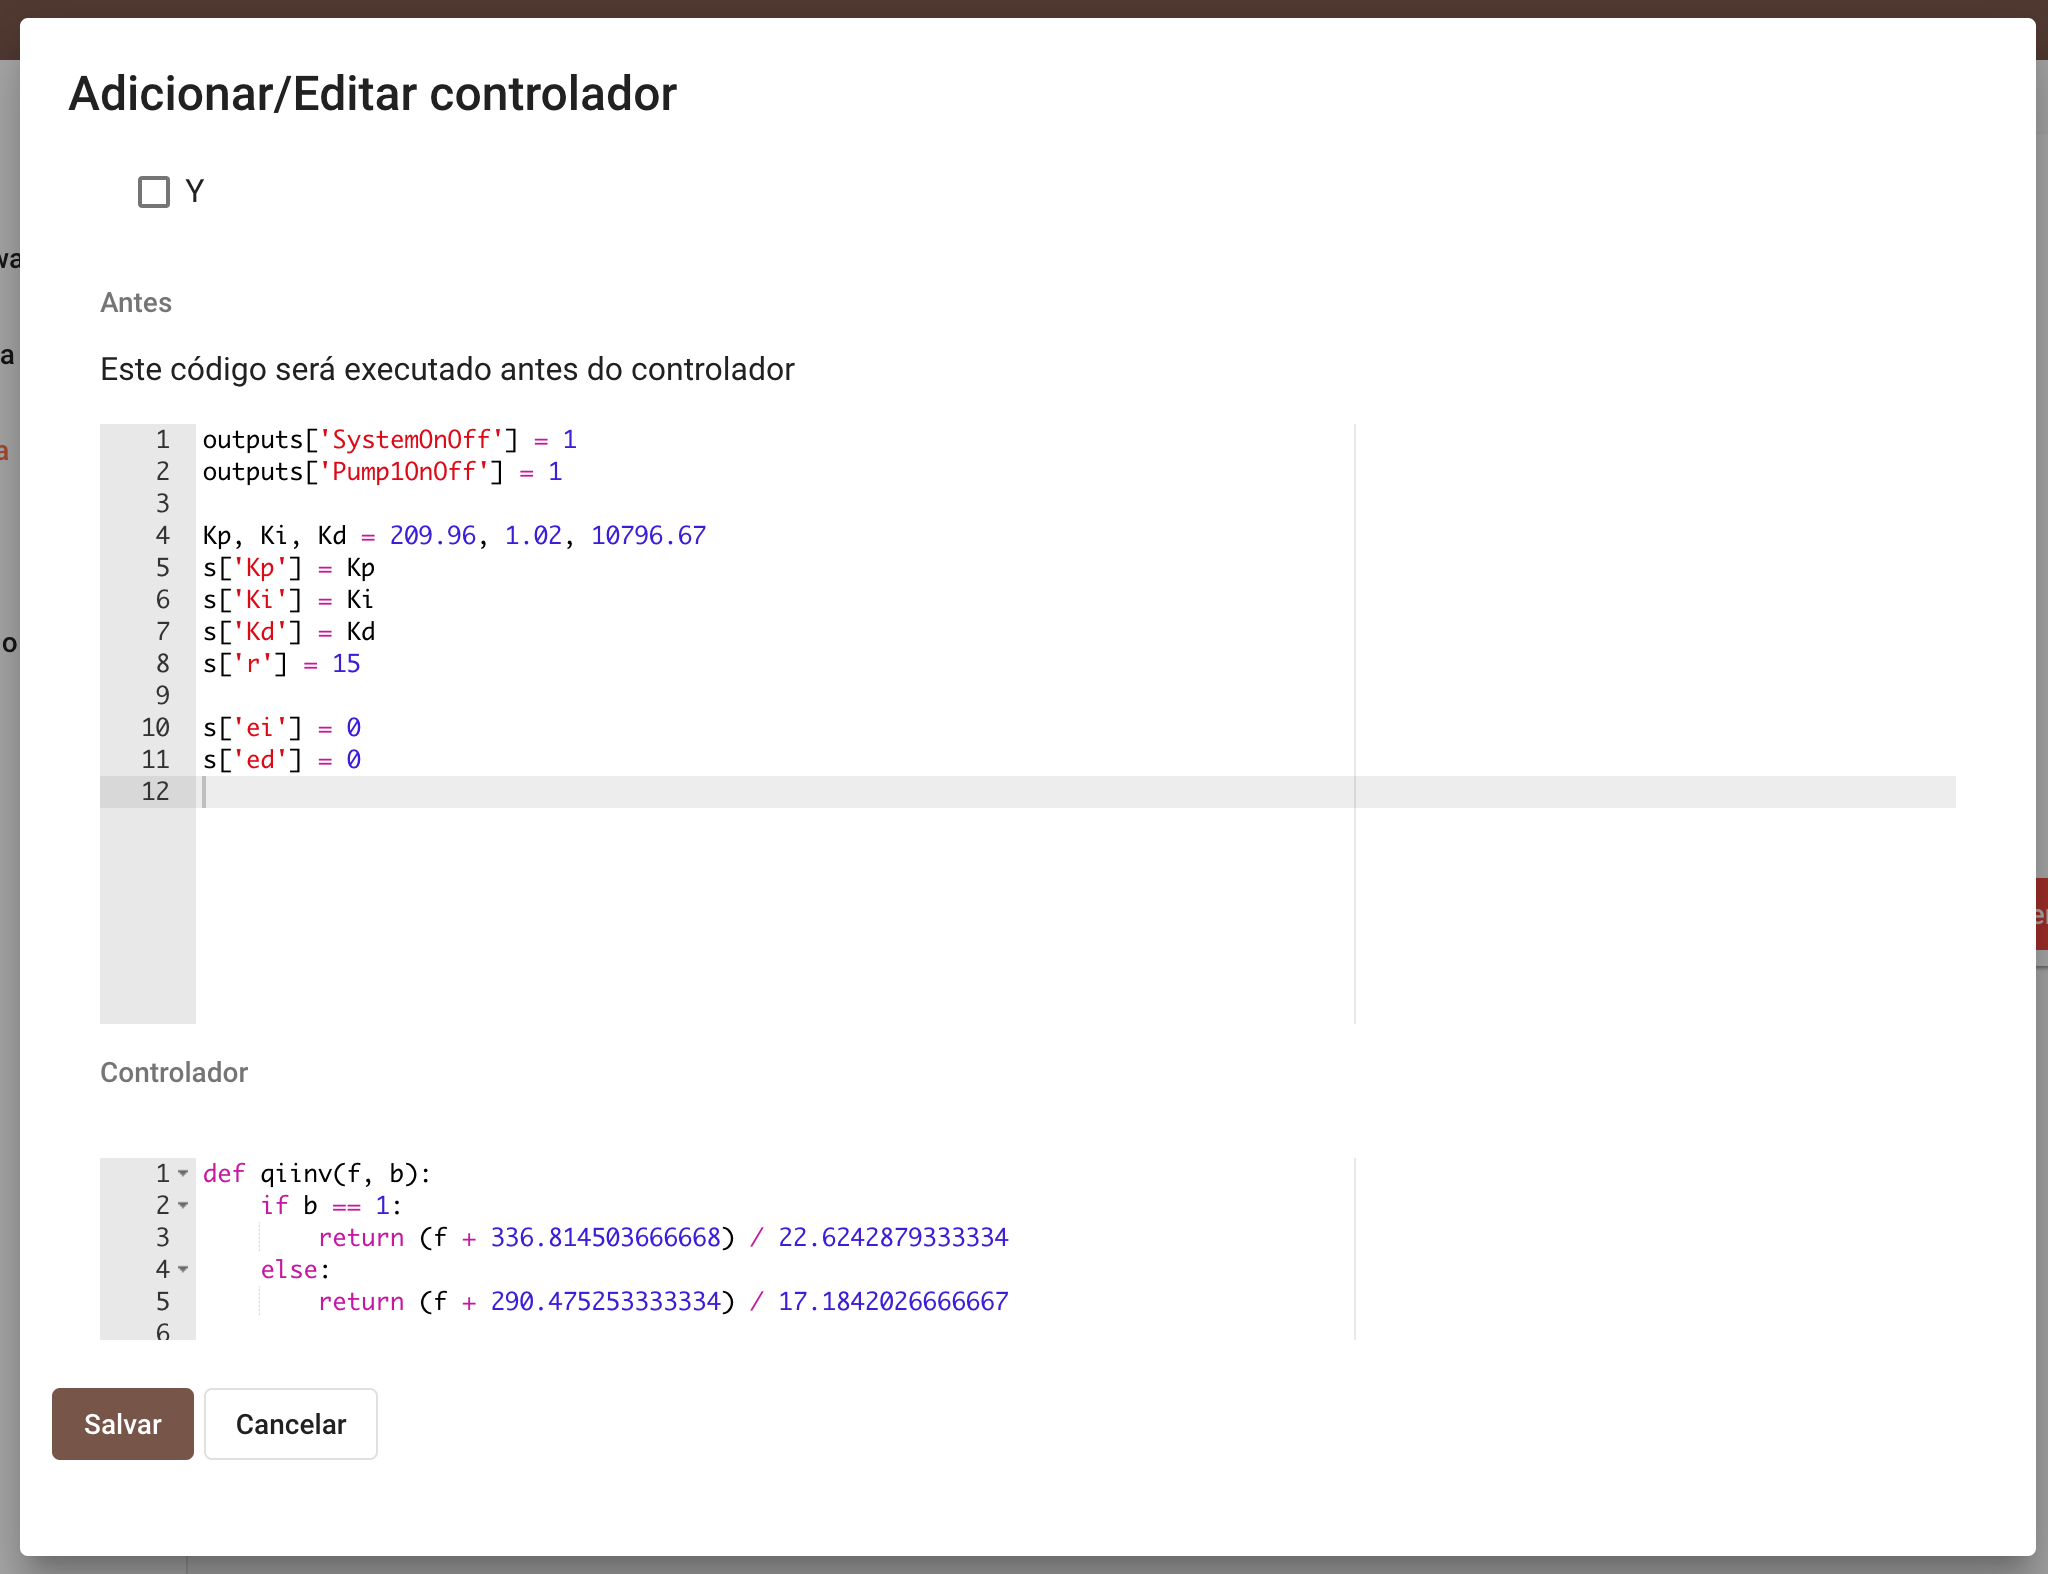
\includegraphics[width=0.9\textwidth]{imgs/control3}
    \caption[Campo \textit{Antes}]{Campo \textit{Antes}}%
    \label{fig:control3}
\end{figure}

Algumas variáveis estão disponíveis nesse campo que o usuário pode fazer uso:

\begin{itemize}
    \item \textbf{inputs} um dicionário com o valor lido na entrada logo antes
                          da execução desse campo. Na Figura~\ref{fig:control2}
                          podemos ver que a entrada \textit{S9} foi selecionada,
                          logo podemos ler seu valor acessando
                          \mintinline{python}{inputs['S9']}.
    \item \textbf{outputs} um dicionário inicialmente vazio. Ao fim da execução
                           desse bloco todas as saídas que forem adicionadas a
                           esse dicionário serão aplicadas no \textit{hardware}.
                           Por exemplo, para ligar a bomba 1 de um sistema,
                           configrada em \textit{Configurações de Hardware} como
                           \textit{Pump1PC} com 40\% de potência, podemos
                           utilizar o código
                           \mintinline{python}{outputs['Pump1PC'] = 40}.
    \item \textbf{s} variável de estado. Essa variável é um dicionário e estará
                     disponível na próxima seção. Ela deve ser usada para
                     persistir dados durante a execução do teste. Por exemplo, o
                     estado atual de um modelo em espaço de estados pode ser
                     salvo nessa variável e alterado posteriormente durante a
                     execução do controlador. É como se fosse uma variável
                     global. Exemplo de uso: \mintinline{python}{s['Kp'] = 1}.
    \item \textbf{dt} o tempo de amostragem.
    \item \textbf{np} a biblioteca numpy já é importada e está disponível sob o
                      nome \textit{np}, não sendo necessário reimportá-la.
    \item \textbf{math} a biblioteca math já é importada, não sendo necessário
                        reimportá-la.
\end{itemize}

No campo \textit{Controlador} (Figura~\ref{fig:control4}) deve-se inserir o
código que será executado a cada \textit{tempo de amostragem} segundos. As
mesmas variáveis disponíveis no campo \textit{Antes} estão disponíveis nesse
campo, além de:

\begin{itemize}
    \item \textbf{t} tempo de execução em segundos.
    \item \textbf{log} todas as entradas e saídas nas variáveis \textbf{inputs}
                       e \textbf{outputs} são salvas e podem ser vistas em
                       gráficos e exportadas para arquivos. A variável
                       \textbf{log} permite fazer a mesma coisa com variáveis
                       que não são entrada ou saída. Por exemplo, pode-se gerar
                       uma entrada para o erro na saída adicionando o erro a
                       esse dicionário, assumindo que o valor da saída anterior
                       esteja salvo como \textit{y\_anterior}:
                       \mintinline{python}{log['erro'] = y - s['y_anterior']}.
                       Na seção \textit{Gráficos}
                       (Capítulo~\ref{chapter:graficos}) a variável
                       \textit{erro} estará disponível nas opções de variáveis
                       de gráficos e de exportação de dados.
\end{itemize}

\begin{figure}[ht!]
    \centering
    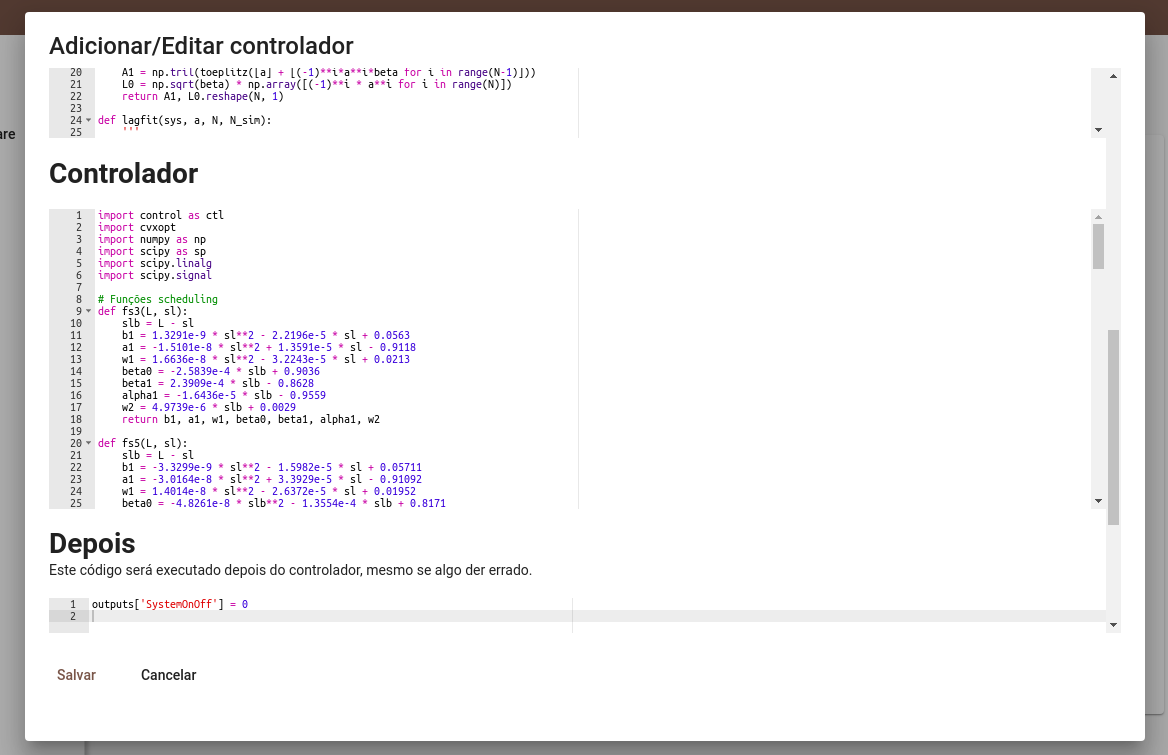
\includegraphics[width=0.9\textwidth]{imgs/control4}
    \caption[Campo \textit{Controlador}]{Campo \textit{Controlador}}%
    \label{fig:control4}
\end{figure}

No campo \textit{Depois} (Figura~\ref{fig:control5}) pode-se inserir código para
desligar o sistema. Esse campo será executado em caso de erro ou caso o teste
execute até o final. Apenas a variável \textit{outputs} está disponível nesse
campo.

\begin{figure}[ht!]
    \centering
    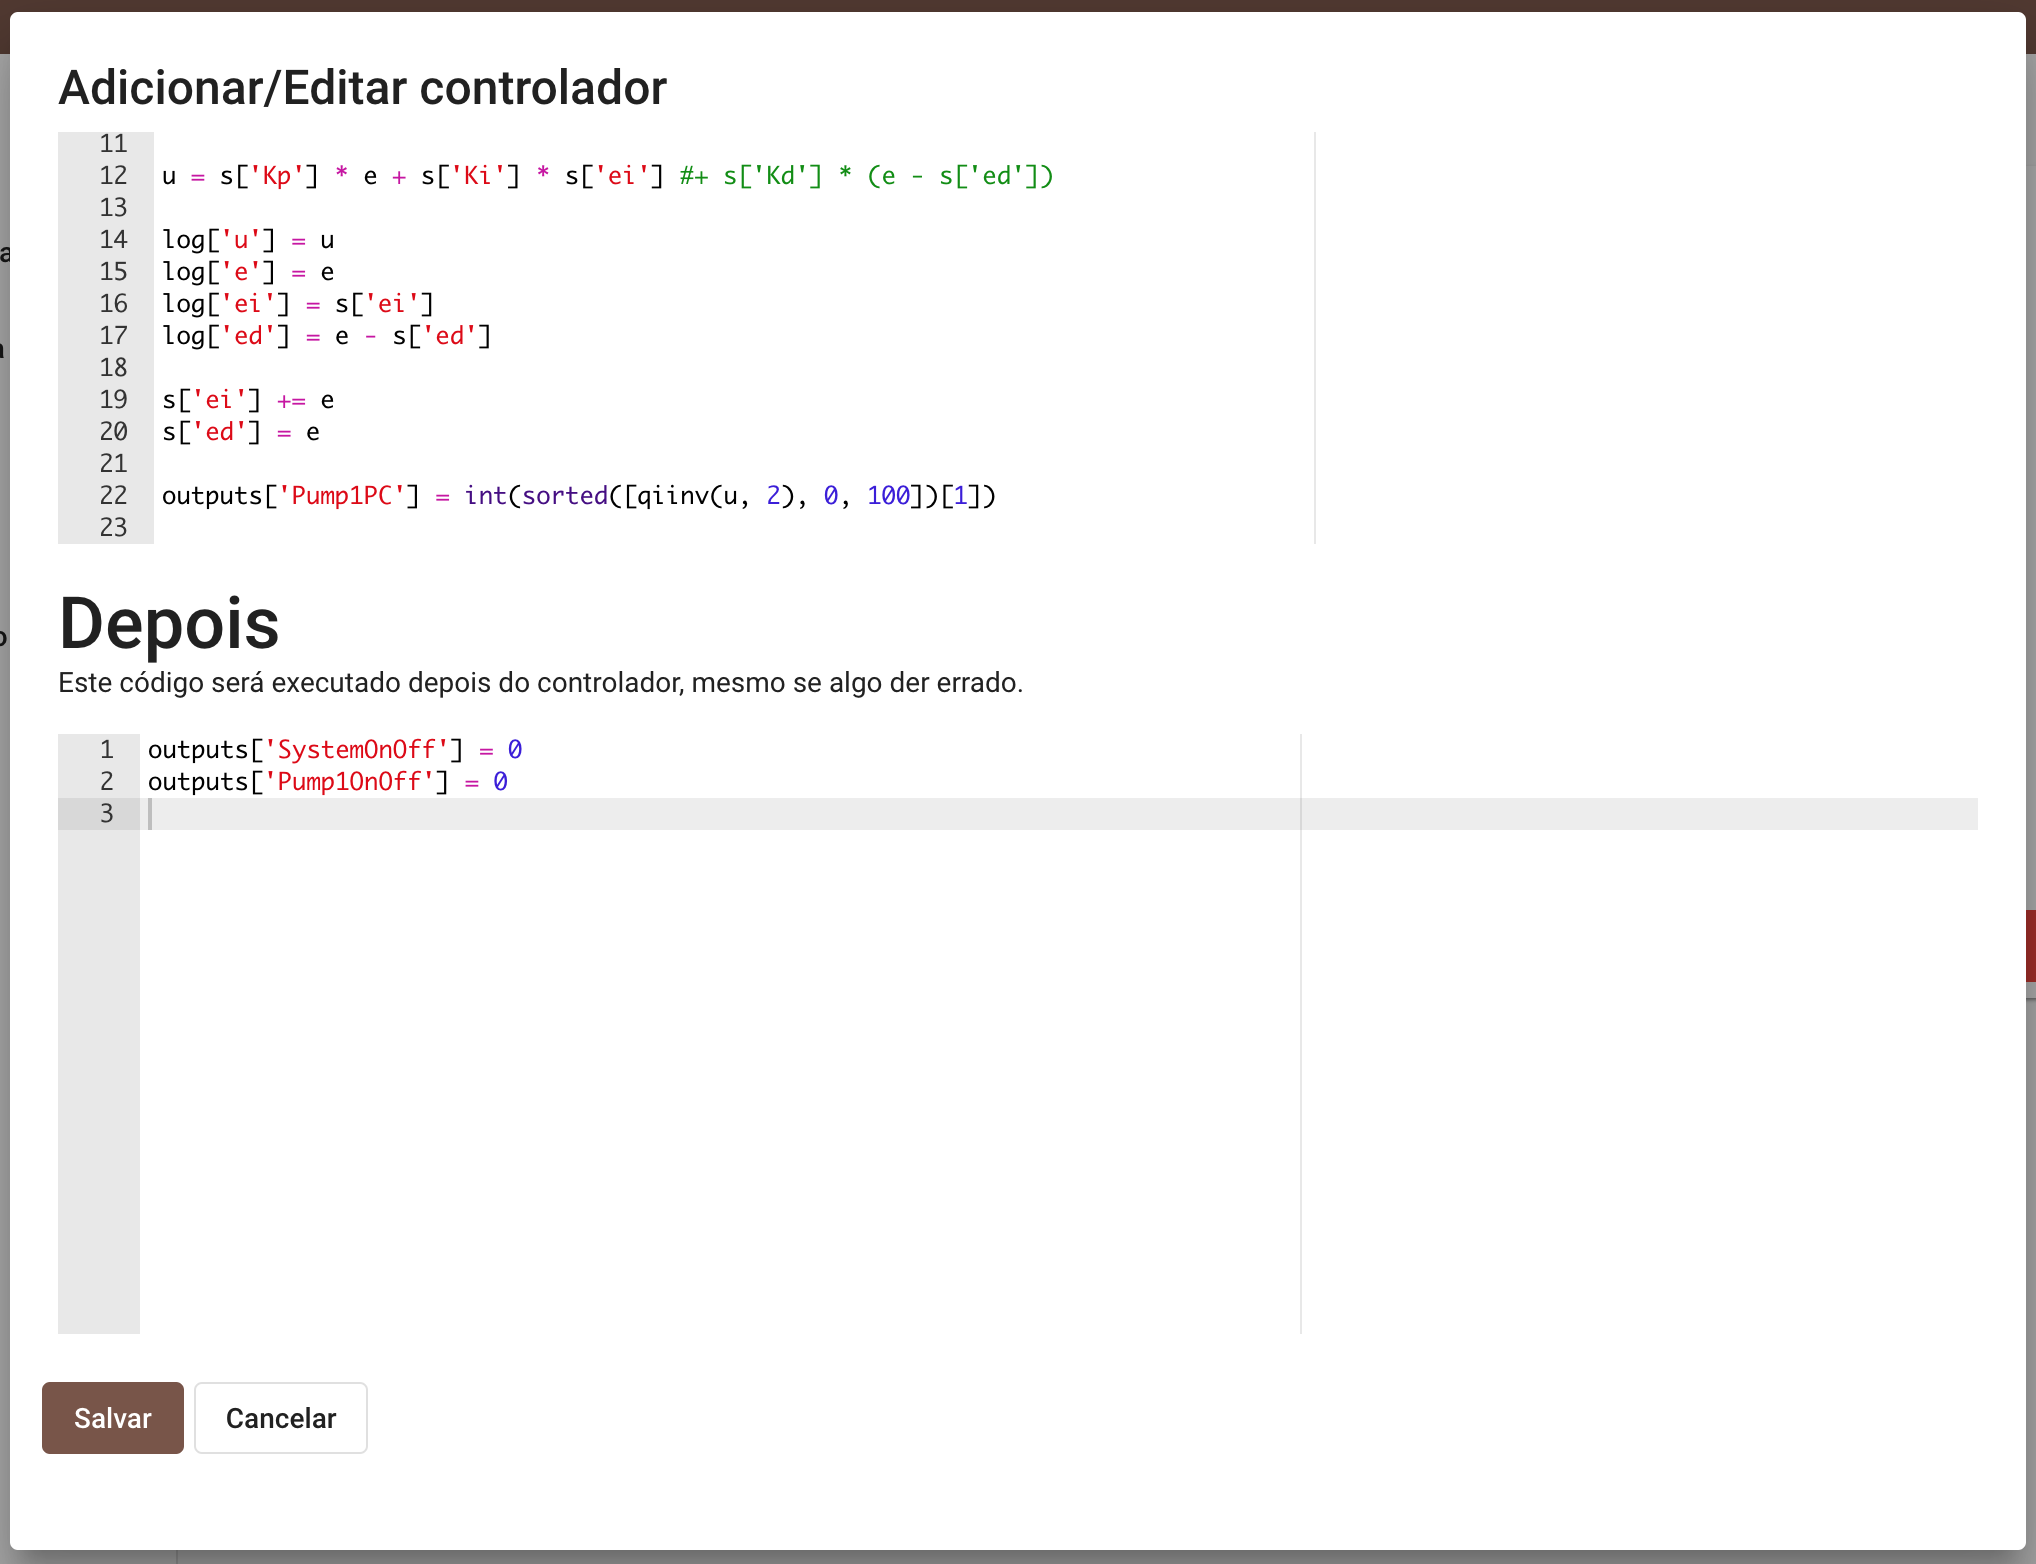
\includegraphics[width=0.9\textwidth]{imgs/control5}
    \caption[Campo \textit{Depois}]{Campo \textit{Depois}}%
    \label{fig:control5}
\end{figure}

O pseudo-código abaixo representa o funcionamento do programa, como se os campos
fossem funções. Obviamente a implementação real é bem mais complexa. Deve-se
chamar atenção ao fato que o controlador será executado sempre num tempo
múltiplo de \textit{dt}. O cálculo do tempo de espera leva em conta o tempo que
foi necessário para executar o código, e sempre aguardará para iniciar a próxima
execução em um múltiplo. Se o tempo de execução do código for menor que
\textit{dt}, então o código sempre executará em \textit{k*dt} segundos. Se o
código levar mais de \textit{dt} segundos para executar, a próxima execução será
agendada para o próximo \textit{k*dt}.

\newpage{}
\begin{pythoncode}
    import math
    import numpy as np

    s = dict()
    outpus = dict()
    inputs = moirai.read_inputs()
    dt = moirai.test_dt()

    s, outputs = user.antes(inputs, outpus, s, dt, math, np)
    
    moirai.write_outputs(outputs)
    
    while True:
        t = moirai.sleep(dt)
        inputs = moirai.read_inputs()
        log = dict()
        outputs = dict()
        
        s, outputs, log = user.controlador(inputs, s, dt, math, np, t, log)

        moirai.write_outputs(outputs)
        moirai.save_variables(inputs, outputs, log)
    
    outpus = dict()
    outputs = user.depois(outputs)
    moirai.write_outputs(outputs)
\end{pythoncode}
